\subsection{Plausibility of embedding space}
tSNE on space
\subsection{PCA on whole corpus}
Repeated 
\subsection{PCA on time-delimited corpora}
Broke out in 50 year periods

\begin{figure}
 \centerline{\framebox{
 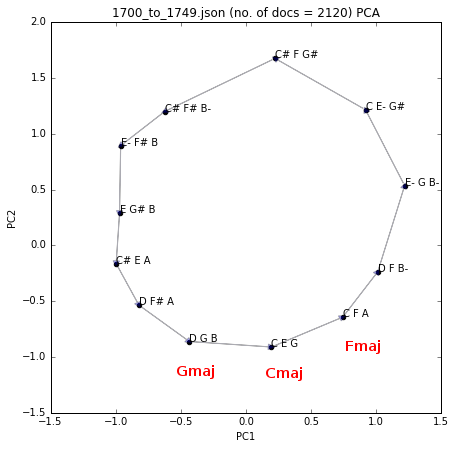
\includegraphics[width=\columnwidth]{figs/1700_majors.png}}}
 \caption{First two eigenvalues for major chords in PCA-reduced embedding space trained on pieces composed between 1700--1749.}
 \label{fig:1700_majors}
\end{figure}

\begin{figure}
 \centerline{\framebox{
 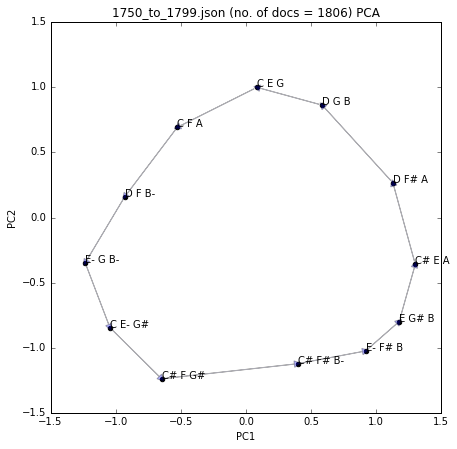
\includegraphics[width=\columnwidth]{figs/1750_majors.png}}}
 \caption{First two eigenvalues for major chords in PCA-reduced embedding space trained on pieces composed between 1750--1799.}
 \label{fig:1750_majors}
\end{figure}


\begin{figure}
 \centerline{\framebox{
 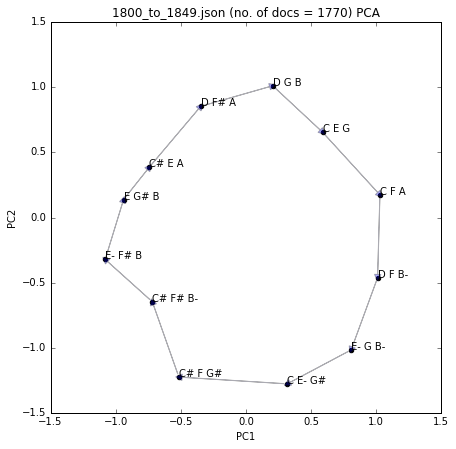
\includegraphics[width=\columnwidth]{figs/1800_majors.png}}}
 \caption{First two eigenvalues for major chords in PCA-reduced embedding space trained on pieces composed between 1800--1849.}
 \label{fig:1800_majors}
\end{figure}


\begin{figure}
 \centerline{\framebox{
 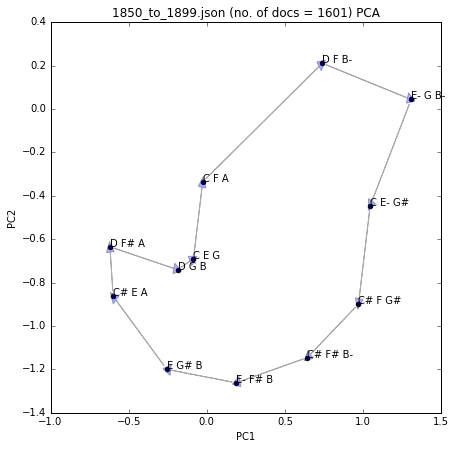
\includegraphics[width=\columnwidth]{figs/1850_majors.png}}}
 \caption{First two eigenvalues for major chords in PCA-reduced embedding space trained on pieces composed between 1850--1899.}
 \label{fig:1850_majors}
\end{figure}

